

\chapter{Multiscale Methods on the Sphere}
\label{ch_mms}

\section{Wavelet Transform on the Sphere}
\label{sect_wts}

\subsection{Isotropic Undecimated Wavelet Transform on the Sphere (UWTS) }
\index{wavelet!undecimated wavelet transform}

There are clearly many different possible implementations of a wavelet transform on the sphere and their performances depend on the application. 
We describe here an undecimated isotropic transform which is similar in many respects to the \emph{ \`a trous} algorithm, and is therefore a good 
candidate for restoration applications. Its isotropy is a favorable property when analyzing a statistically isotropic Gaussian field such as the 
CMB, or data sets such as maps of galaxy clusters, which contain only isotropic features~\cite{starck:book98}. Our isotropic transform is obtained 
using a scaling function $\phi_{l_c}(\vartheta, \varphi)$ with cut-off frequency $l_c$ and azimuthal symmetry, meaning that $\phi_{l_c}$ does not 
depend on the azimuth $\varphi$. Hence the spherical harmonic coefficients $\hat \phi_{l_c} (l,m)$ of $\phi_{l_c}$ vanish when $m \ne 0$ so that :
\begin{eqnarray}
\phi_{l_c}(\vartheta, \varphi)= \phi_{l_c}(\vartheta) = \sum_{l = 0}^{l = l_c} \hat \phi_{l_c} (l,0) Y_{l,0}(\vartheta, \varphi)
\end{eqnarray}
where the $Y_{l,m}$ are the spherical harmonic basis functions. Then, convolving a map $f(\vartheta, \varphi)$ with $\phi_{l_c}$ is greatly simplified 
and the spherical harmonic coefficients $\hat c_{0}(l,m)$ of the resulting map $c_0(\vartheta, \varphi)$ are readily given by \cite{bogdanova}:
\begin{eqnarray}\label{eq:conv}
 \hat c_{0}(l,m) = \widehat{\phi_{l_c} * f} (l,m) = \sqrt{\frac{4\pi}{2l+1} } \hat \phi_{l_c} (l,0) \hat f(l,m) 
\end{eqnarray}
where $*$ stands for convolution.

\subsubsection*{From one resolution to the next one}

A sequence of smoother approximations of $f$ on a dyadic resolution scale can be obtained using the scaling function $\phi_{l_c}$ as follows
\begin{eqnarray}
c_0   & = &  \phi_{ l_{c} }  * f    \nonumber    \\
c_1   & = &  \phi_{2^{-1} l_{c} }   * f    \nonumber	   \\
&\ldots&\nonumber\\ 
c_j    &=&   \phi_{2^{-j}  l_{c}  }  * f  \nonumber    \\
\end{eqnarray}
where $\phi_{2^{-j} l_{c} }$ is a rescaled version of $\phi_{l_{c}}$ with cut-off frequency $2^{-j} l_{c}$. The above multi-resolution sequence 
can actually be obtained recursively. Define a low pass filter $h_{j}$ for each scale $j$ by 
%\begin{eqnarray}
 %\hat h_{j}(l,m) = \left\{
%  \begin{array}{ll}
 % \frac {   \hat \phi_{\frac{l_{c}}{2^{j+1}} }(l,m)   }   {  \hat  \phi_{  \frac{l_{c}}{2^{j}} }(l,m)   } & \mbox{if }  l  < \frac{ l_{c}} {2^{j+1}} \\
%0 & \mbox{otherwise } \ 
 % \end{array}
  %\right.
%\end{eqnarray}
\begin{eqnarray}
 \hat{H}_{j}(l,m) = \sqrt{\frac{4\pi}{2l+1} }  \hat h_{j}(l,m) = \left\{
  \begin{array}{ll}
  \frac {   \hat \phi_{\frac{l_{c}}{2^{j+1}} }(l,m)   }   {  \hat  \phi_{  \frac{l_{c}}{2^{j}} }(l,m)   } & \mbox{if }  l  < \frac{ l_{c}} {2^{j+1}} \quad \textrm{and}\quad m = 0\\
0 & \mbox{otherwise } \ 
  \end{array}
  \right.
\end{eqnarray}
It is then easily shown that $c_{j+1}$ derives from $c_j$ by convolution with $h_j$:  $c_{j+1} = c_{j} * h_j$.

\subsubsection*{The wavelet coefficients}

Given an asymmetrical wavelet function $\psi_{l_c}$, we can derive in the same way a high pass filter $g_j$ on each scale $j$:
%\begin{eqnarray}
%\hat{g}_{j}(l,m) = \left\{
%  \begin{array}{ll}
%  \frac{\hat{\psi}_{2l_{c}}}{\hat{\phi}_{l_{c}}} & \mbox{if }  l  < l_{c} \\
%1 & \mbox{otherwise } \ 
%  \end{array}
%  \right.
%\end{eqnarray}
\begin{eqnarray}
 \hat{G}_{j}(l,m) = \sqrt{\frac{4\pi}{2l+1} }  \hat{g}_{j}(l,m) = \left\{
  \begin{array}{ll}
 \frac {   \hat \psi_{\frac{l_{c}}{2^{j+1}} }(l,m)   }   {  \hat  \phi_{  \frac{l_{c}}{2^{j}} }(l,m)   } & \mbox{if }  l  < \frac{ l_{c}} {2^{j+1}} \quad \textrm{and}\quad m = 0\\ 
1 &\mbox{if }  l  \ge \frac{ l_{c}} {2^{j+1}} \quad \textrm{and}\quad m = 0\\ 
0&  \mbox{otherwise }\
  \end{array}
  \right.
\end{eqnarray}
Using these, the wavelet coefficients $w_{j+1} $ at scale $j+1$ are obtained from the previous resolution by a simple convolution: $w_{j+1} = c_{j} * g_j$.\\

Just as with the \emph{\`a trous} algorithm, the wavelet coefficients can be defined as the difference between two consecutive resolutions, 
$w_{j+1}(\vartheta, \varphi) = c_{j}(\vartheta, \varphi) - c_{j+1}(\vartheta, \varphi)$, which in fact corresponds to making the following 
specific choice for the wavelet function $\psi_{l_c}$:
\index{wavelet!\`a trous}
%\begin{eqnarray}
%\hat \psi(l,m) = \hat \phi_{l_c} (l,m)  - \hat \phi_{l_c/2}(l,m)
%\end{eqnarray}
\begin{eqnarray}
\hat \psi_{\frac{l_c}{2^{j}}}(l,m) = \hat \phi_{\frac{l_c}{2^{j-1}}} (l,m)  - \hat \phi_{\frac{l_c}{2^{j}}}(l,m)
\end{eqnarray}
The high pass filters $g_j$ defined above are, in this particular case, expressed as: 
%\begin{eqnarray}
%\hat{g}_{j}(l,m) =  1 - \hat{h}_j(l,m)  
%\end{eqnarray}
\begin{eqnarray}
 \hat{G}_{j}(l,m) = \sqrt{\frac{4\pi}{2l+1} } \hat{g}_{j}(l,m) =  1 - \sqrt{\frac{4\pi}{2l+1} } \hat{h}_j(l,m)   =   1 - \hat{H}_j(l,m) 
\end{eqnarray}
Obviously, other wavelet functions could be used just as well.


\subsubsection*{Choice of the scaling function}
\index{scaling function}
Any function with a cut-off frequency is a possible candidate. We retained here a B-spline function of order 3. It is quite similar to a 
Gaussian function and converges rapidly to $0$:
%\begin{eqnarray}
%\hat \phi_{l_c} (l,m) =\frac{3}{2} B_{3\ \frac{l}{l_{c}}m}
%\end{eqnarray}
\begin{eqnarray}
\hat \phi_{l_c} (l,m = 0) =\frac{3}{2} B_{3}( \frac{2 l}{l_{c} })  % \quad \textrm{where} \quad   B_3(x) = \frac{1}{12}({\mid{x-2}\mid}^3 - 4 {\mid{x-1}\mid}^3 + 6 {\mid{x}\mid}^3 - 4 {\mid{x+1}\mid}^3 + {\mid{x+2}\mid}^3)
\end{eqnarray}
where $B(x) = \frac{1}{12}({\mid{x-2}\mid}^3 - 4 {\mid{x-1}\mid}^3 + 6 {\mid{x}\mid}^3 - 4 {\mid{x+1}\mid}^3 + {\mid{x+2}\mid}^3)$.

\begin{figure*}[htb]
\centerline{
\hbox{
% \psfig{figure=ch1_diff_uv_phi_psi.ps,bbllx=0.5cm,bblly=13.5cm,bburx=20.5cm,bbury=27cm,height=5cm,width=14.5cm,clip=}
\psfig{figure=fig_sphere_filterbank.pdf,bbllx=2cm,bblly=21cm,bburx=20cm,bbury=26cm,height=7cm,width=14.5cm,clip=}
}}
\caption{On the left, the scaling function $\hat{\phi}$ and, on the 
right, the wavelet function $\hat{\psi}$.}
\label{fig_diff_uv_phi_psi}
\end{figure*}

In Fig.~\ref{fig_diff_uv_phi_psi} the chosen scaling function derived from a $B$-spline of degree 3, and its resulting wavelet function, are plotted in frequency space.
\index{B-spline}


\begin{center}
\begin{tabular}{|c|} \hline
\begin{minipage}[b]{5.3in}
\vspace{0.1in}

\small{
\textsf{1. Compute the $B_3$-spline scaling function and derive $\psi$, $h$ and $g$ numerically.}

\textsf{2. Compute the corresponding Spherical Harmonics of image $c_0$. We get ${\hat c}_0$.}

\textsf{3. Set $j$ to $0$. Iterate:}

\hspace{0.3in} \textsf{4. Multiply  $\hat{c}_j$ by $\widehat H_{j}$. We get the array $\hat{c}_{j+1}$.}

\hspace{0.33in} \textsf{Its inverse Spherical Harmonics Transform gives the image at scale $j+1$.}

\hspace{0.3in} \textsf{5. Multiply $\hat{c}_j$ by $\widehat G_{j}$. We get the complex array
$\hat{w}_{j+1}$.}

\hspace{0.33in} \textsf{ The inverse Spherical Harmonics transform of $\hat{w}_{j+1}$ 
gives the wavelet coefficients $w_{j+1}$ at scale $j+1$.}

\hspace{0.3in} \textsf{6. j=j+1 and if $j \leq  J$, return to Step 4.}

\textsf{9. The set $\{w_1, w_2, \dots, w_{J}, c_{J}\}$ describes the wavelet transform on the sphere of $c_0$.}}

\vspace{0.05in}
\end{minipage}
\\\hline
\end{tabular}
\\ \vspace{0.1in}
The numerical algorithm for the undecimated wavelet transform on the sphere.
\end{center}
\linespread{1.3}
\index{algorithm!undecimated wavelet transform}

If the wavelet is the difference between two resolutions, Step 5 in the above UWTS algorithm can be replaced by the following simple subtraction $w_{j+1} = c_{j} - c_{j+1}$.

\subsubsection*{Reconstruction}
\index{wavelet!undecimated wavelet reconstruction}
When the wavelet is the difference between two resolutions, the reconstruction of an image from its wavelet coefficients ${\cal W} = \{w_1,\dots, w_{J}, c_{J}\}$ is straightforward: 
\begin{eqnarray}
 c_{0}(\theta, \phi) = c_{J}(\theta, \phi) + \sum_{j=1}^J  w_j(\theta, \phi)
\end{eqnarray}
This is the same reconstruction formula as in the \emph{\`a trous} algorithm: the simple sum of all scales reproduces the original data. 
Actually, since the present decomposition is redundant, the procedure for reconstructing an image from its coefficients is not unique and 
in fact this can profitably be used to impose additional constraints on the synthesis functions (\emph{e.g.} smoothness, positivity) used 
in the reconstruction. Here for instance, using the relations:
\begin{eqnarray}
\hat c_{j+1}(l,m) = \widehat H_{j} (l,m)  \hat c_{j} (l,m) \nonumber \\
\hat w_{j+1}(l,m) = \widehat G_{j} (l,m) \hat c_{j} (l,m) 
\end{eqnarray}
a least squares estimate of $c_j$ from $c_{j+1}$ and $w_{j+1}$ gives:
\begin{eqnarray}
%c_{j}   = c_{j+1}  * {\tilde h}_{2^{j}l_{c}}   + w_{j+1}  * {\tilde g}_{2^{j}l_{c}}
\hat{c}_{j}   = \hat{c}_{j+1}  {\widehat {\tilde H}}_{j}   + \hat{w}_{j+1}  {\widehat {\tilde G}}_{j} 
\end{eqnarray}
where the conjugate filters $ {\widehat {\tilde H}}_j $ and $ {\widehat {\tilde G}}_j$ have the expression:
\begin{eqnarray}
 {\widehat {\tilde H}}_j =  \sqrt{\frac{4\pi}{2l+1} } {\hat {\tilde h}}_j & = {\widehat H}_{j}^* /
(\mid {\widehat H}_{j}\mid^2 + \mid {\widehat G}_j\mid^2) \label{eqnht} \\ 
 {\widehat {\tilde G}}_j =  \sqrt{\frac{4\pi}{2l+1} } {\hat {\tilde g}}_j & = {\widehat G}_{j}^* /
(\mid {\widehat H}_j \mid^2 + \mid {\widehat G}_j \mid^2)
\label{eqngt}
\end{eqnarray}
%\begin{eqnarray}
%{\hat {\tilde h}} & = {\hat h^* /
%(\mid \hat h\mid^2 + \mid \hat g\mid^2}) \label{eqnht} \\ 
%{\hat {\tilde g}} & = {\hat g^* /
%(\mid \hat h \mid^2 + \mid \hat g \mid^2})
%\label{eqngt}
%\end{eqnarray}
and the reconstruction algorithm is:
\begin{center}
\begin{tabular}{|c|} \hline
\begin{minipage}[b]{5.3in}
\vspace{0.1in}

\small{
\textsf{1. Compute the $B_3$-spline scaling function and derive $\hat \psi$, $\hat h$, $\hat g$, ${\hat {\tilde h}}$, ${\hat {\tilde g}}$ numerically.}

\textsf{2. Compute the corresponding Spherical Harmonics of the image at the low resolution $c_J$. We get ${\hat c}_J$.}

\textsf{3. Set $j$ to $J-1$. Iterate:}

\hspace{0.3in} \textsf{4. Compute the Spherical Harmonics transform of the wavelet coefficients $w_{j+1}$ at scale $j+1$. We get  $\hat{w}_{j+1}$.}

\hspace{0.3in} \textsf{5. Multiply  $\hat{c}_{j+1}$ by ${\widehat {\tilde H}}_j $.}

\hspace{0.3in} \textsf{6. Multiply $\hat{w}_{j+1}$ by $ {\widehat {\tilde G}}_j $.}

\hspace{0.3in} \textsf{7. Add the results of steps 6 and 7. We get $\hat  c_j$.}

\hspace{0.3in} \textsf{8. j=j-1 and if $j \ge  0$, return to Step 4.}

\textsf{9. Compute The inverse Spherical Harmonic transform of $\hat  c_0$}}

\vspace{0.05in}
\end{minipage}
\\\hline
\end{tabular}
\\ \vspace{0.1in}
% The numerical algorithm for the inverse wavelet transform on the sphere.
\end{center}
\linespread{1.3}
\index{algorithm!undecimated wavelet reconstruction}
The synthesis low pass and high pass filters $\hat{\tilde h}$ and $\hat{\tilde g}$ are plotted in Fig.~\ref{fig_diff_uv_ht_gt}. 

\begin{figure*}[htb]
\centerline{
\hbox{
% \psfig{figure=ch1_diff_uv_ht_gt.pdf,bbllx=0.5cm,bblly=13.5cm,bburx=20.5cm,bbury=27cm,height=5cm,width=14.5cm,clip=}
\psfig{figure=fig_sphere_filterbank.pdf,bbllx=2cm,bblly=12.5cm,bburx=20cm,bbury=16.7cm,height=7cm,width=14.5cm,clip=}
}}
\caption{On the left, the filter $\hat{\tilde{h}}$, and on the right the 
filter $\hat{\tilde{g}}$.}
\label{fig_diff_uv_ht_gt}
\end{figure*}


\begin{figure*}
\vbox{
\centerline{
\hbox{
 % \psfig{figure=fig_uwt_sphere.ps,bbllx=1cm,bblly=7cm,bburx=17cm,bbury=22cm,height=9cm,width=12cm,clip=}
\psfig{figure=fig_wmap_bw.pdf,bbllx=0.5cm,bblly=9.5cm,bburx=20.5cm,bbury=20cm,width=8cm,height=4.5cm,clip=}
\psfig{figure=fig_wmap_scale1_bw.pdf,bbllx=0.5cm,bblly=9.5cm,bburx=20cm,bbury=20cm,width=8cm,height=4.5cm,clip=}
}}
\centerline{
\hbox{
\psfig{figure=fig_wmap_scale2_bw.pdf,bbllx=0.5cm,bblly=9.5cm,bburx=20cm,bbury=20cm,width=8cm,height=4.5cm,clip=}
\psfig{figure=fig_wmap_scale3_bw.pdf,bbllx=0.5cm,bblly=9.5cm,bburx=20cm,bbury=20cm,width=8cm,height=4.5cm,clip=}
}}
\centerline{
\hbox{
\psfig{figure=fig_wmap_scale4_bw.pdf,bbllx=0.5cm,bblly=9.5cm,bburx=20cm,bbury=20cm,width=8cm,height=4.5cm,clip=}
\psfig{figure=fig_wmap_scale5_bw.pdf,bbllx=0.5cm,bblly=9.5cm,bburx=20cm,bbury=20cm,width=8cm,height=4.5cm,clip=}
}}
}
\caption{{ WMAP Data and its wavelet transform on the Sphere using five resolution levels (4 wavelet scales and the coarse scale). 
The sum of these five maps reproduces exactly the original data (top left). Top,original data and the first wavelet scale. Middle, 
the second and third wavelet scales. Bottom, the fourth wavelet scale and the last smoothed array.}}
\label{Figure:UWTS}
\end{figure*}


\begin{figure}
\centerline{
\hbox{
% \centering
% 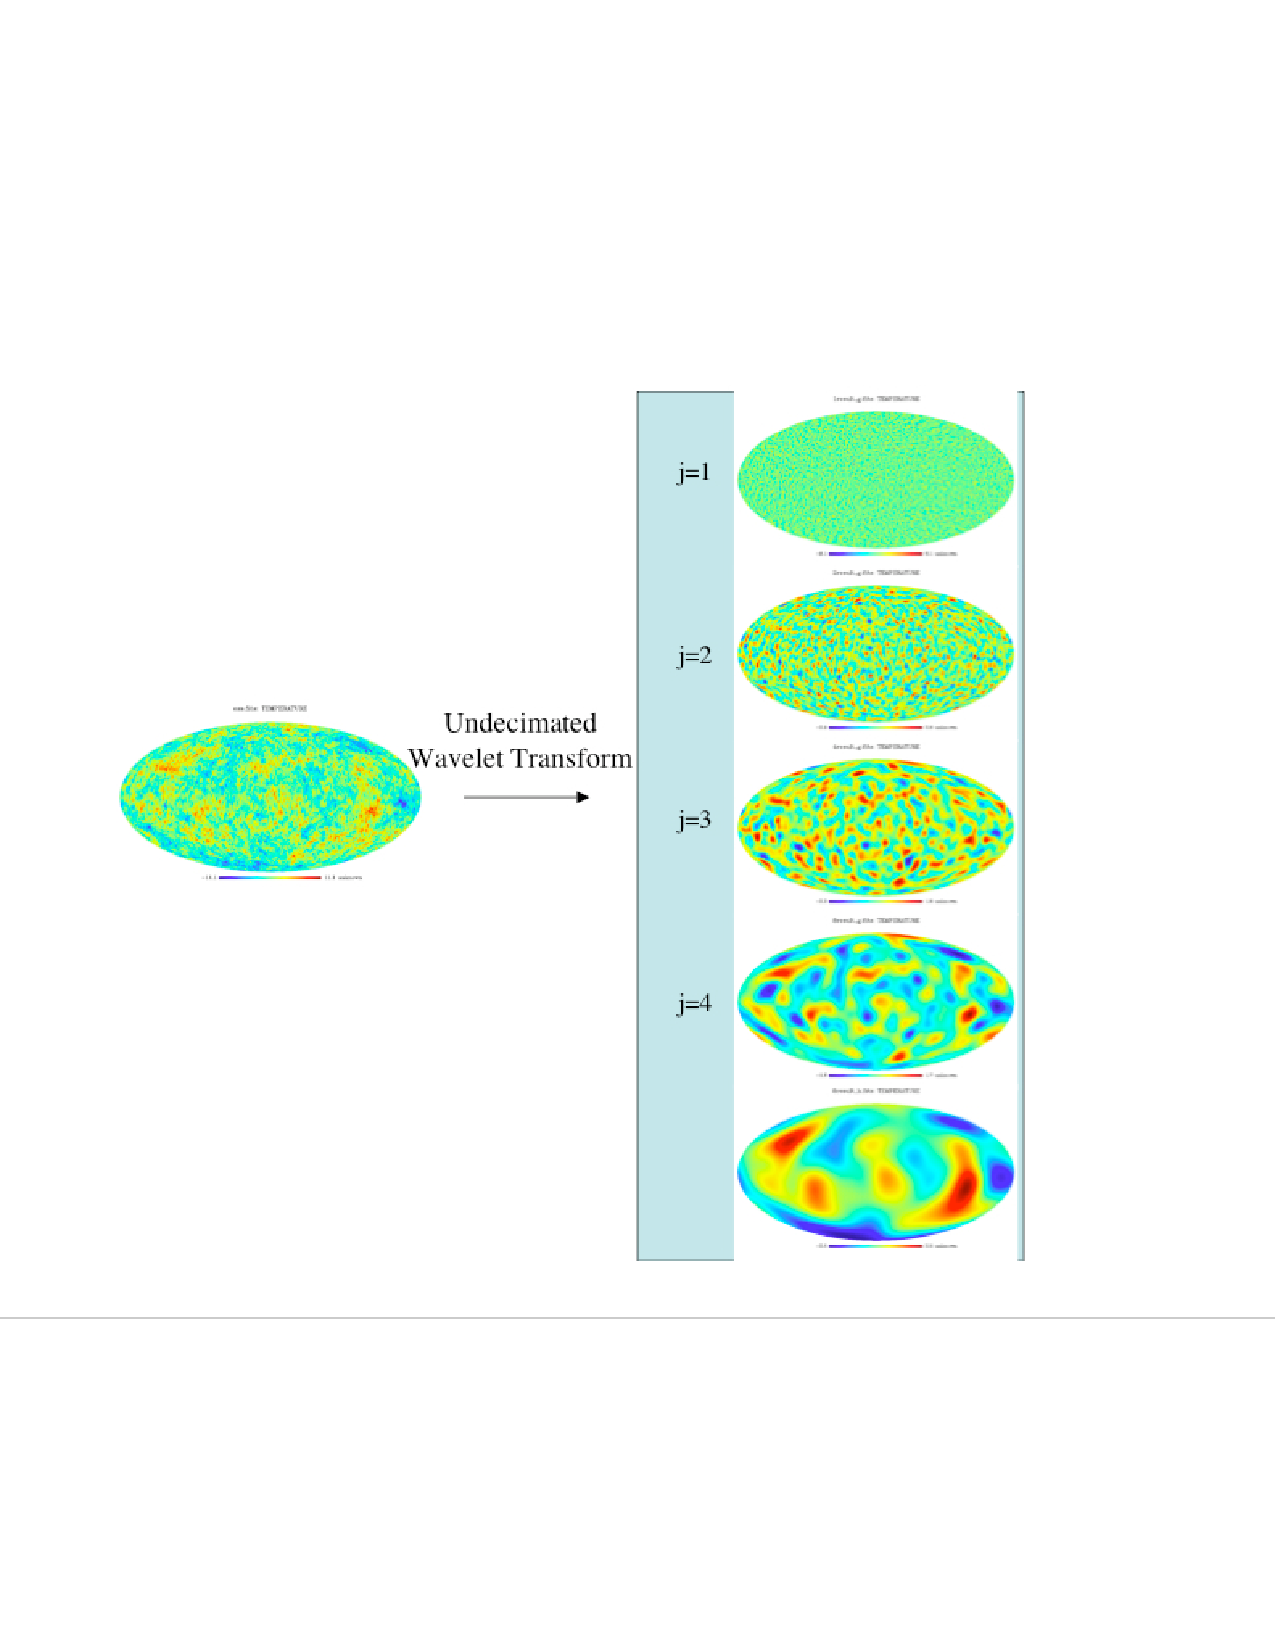
\includegraphics[height=8truecm,width=6truecm]{fig_uwt_sphere.pdf}
% 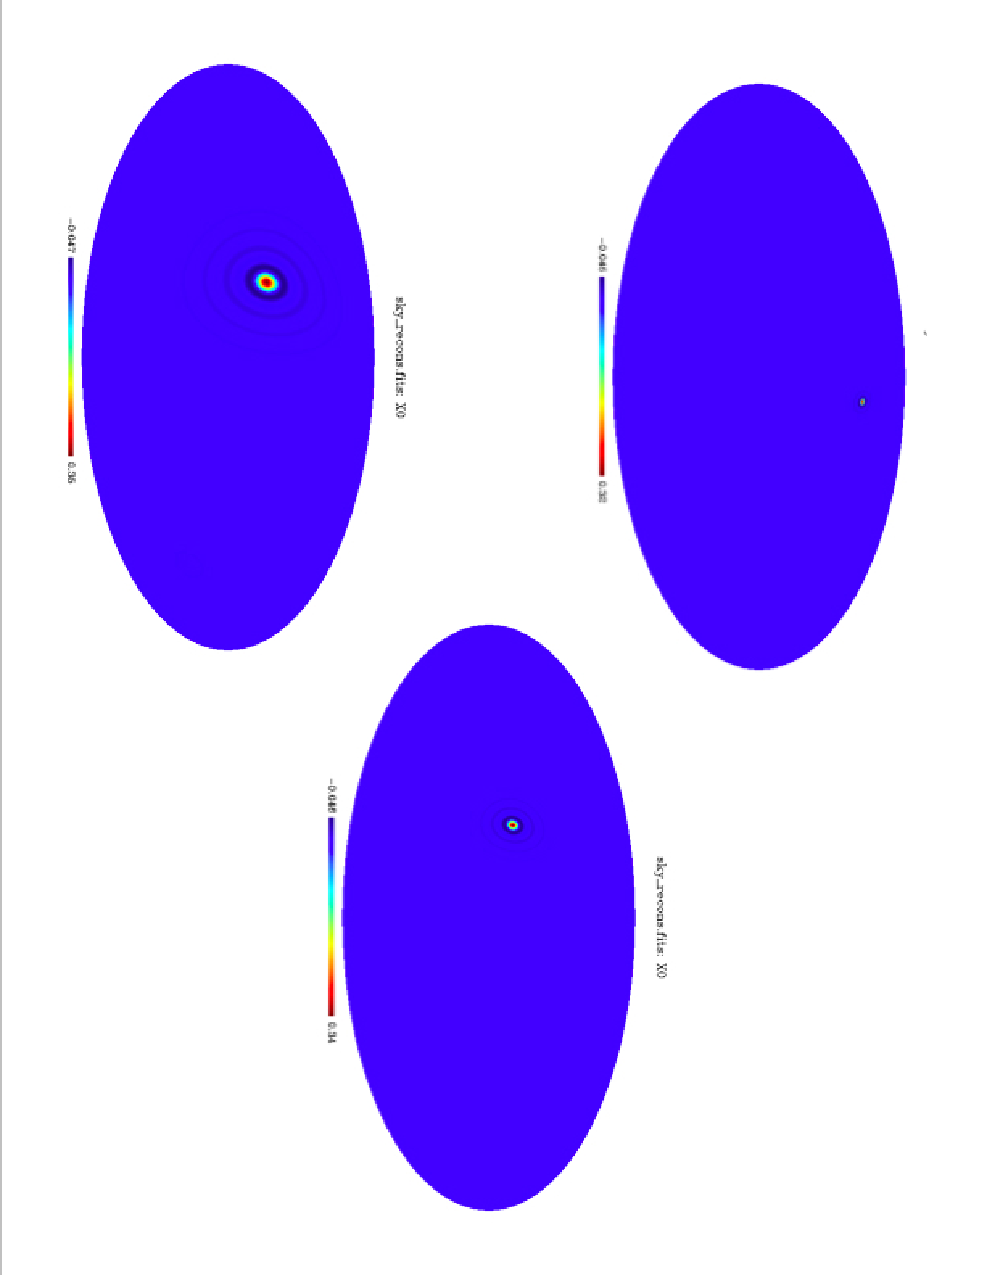
\includegraphics[height = 6 in]{fig_backwt_sphere.pdf}
\psfig{figure=fig_backwt_sphere.pdf,bbllx=0.5cm,bblly=6.5cm,bburx=20.5cm,bbury=21.5cm,height=7.5cm,width=10cm,clip=}
}}
\caption{{ Backprojection of a wavelet coefficient at different scales. Each map is obtained by setting all wavelet coefficients 
to zero but one, and applying an inverse wavelet transform. Depending on the scale and the position of the non zero wavelet coefficient, 
the reconstructed image presents an isotropic feature with a given size.}}
\label{Figure:back_wt}
\end{figure}

{ Figure~\ref{Figure:UWTS} shows the WMAP data (top left) and its undecimated wavelet decomposition on the sphere using 
five resolution levels. Figures~\ref{Figure:UWTS} top right, middle left, middle right and bottom left show respectively 
the four wavelet scales. Figure~\ref{Figure:UWTS} bottom right shows the last smoothed array. Figure~\ref{Figure:back_wt} 
shows the backprojection of a wavelet coefficient at different scales and positions.}

\subsection{Isotropic Pyramidal Wavelet Transform on the Sphere (PWTS) }
\index{wavelet!pyramidal wavelet transform}
\index{wavelet!pyramidal wavelet reconstruction}

\begin{figure*}
\vbox{
\centerline{
\hbox{
 % \psfig{figure=fig_pyrwt_sphere.ps,bbllx=1cm,bblly=7cm,bburx=17cm,bbury=22cm,height=9cm,width=12cm,clip=}
\psfig{figure=fig_wmap_bw.pdf,bbllx=0.5cm,bblly=9.5cm,bburx=20.5cm,bbury=20cm,width=8cm,height=4.5cm,clip=}
\psfig{figure=fig_wmap_pscale1_bw.pdf,bbllx=0.5cm,bblly=9.5cm,bburx=20cm,bbury=20cm,width=8cm,height=4.5cm,clip=}
}}
\centerline{
\hbox{
\psfig{figure=fig_wmap_pscale2_bw.pdf,bbllx=0.5cm,bblly=9.5cm,bburx=20cm,bbury=20cm,width=8cm,height=4.5cm,clip=}
\psfig{figure=fig_wmap_pscale3_bw.pdf,bbllx=0.5cm,bblly=9.5cm,bburx=20cm,bbury=20cm,width=8cm,height=4.5cm,clip=}
}}
\centerline{
\hbox{
\psfig{figure=fig_wmap_pscale4_bw.pdf,bbllx=0.5cm,bblly=9.5cm,bburx=20cm,bbury=20cm,width=8cm,height=4.5cm,clip=}
\psfig{figure=fig_wmap_pscale5_bw.pdf,bbllx=0.5cm,bblly=9.5cm,bburx=20cm,bbury=20cm,width=8cm,height=4.5cm,clip=}
}}
}
\caption{{ WMAP Data (top left) and its pyramidal wavelet transform on the Sphere using five resolution levels (4 wavelet scales 
and the coarse scale). The original map can be reconstructed exactly from the pyramidal wavelet coefficients.Top, original data 
and the first wavelet scale. Middle, the second and third wavelet scales. Bottom, the fourth wavelet scale and the last smoothed 
array. The number of pixels is divided by four at each resolution level, which can be helpful when the data set are large.}}
\label{Figure:PWTS}
\end{figure*}

In the previous algorithm, no downsampling is performed and each scale of the wavelet decomposition has the same number of pixels as 
the original data set. Therefore, the number of pixels in the decomposition is equal to the number of pixels in the data multiplied 
by the number of scales. For applications such as PLANCK data restoration, we may prefer to introduce a decimation in the decomposition 
so as to reduce the required memory size and the computation time. This can be done easily by using a specific property of the chosen 
scaling function. Indeed, since we are considering here a scaling function with an initial cut-off $l_c$ in spherical harmonic multipole 
number $l$, and since the actual cut-off is reduced by a factor of two at each step, the number of significant spherical harmonic 
coefficients is then reduced by a factor of four after each convolution with the low pass filter $h$. Therefore, we need less pixels 
in the direct space when we compute the inverse spherical harmonic transform. Using the Healpix pixelization scheme \cite{healpix}, 
this can be done easily by dividing by 2 the {\it nside} parameter when calling to the inverse spherical harmonic transform routine.

{ Figure~\ref{Figure:PWTS} shows WMAP data (top left) and its pyramidal wavelet transform using five scales. As the scale number increases 
(i.e. the resolution decreases), the pixel size becomes larger. Figures~\ref{Figure:PWTS} top right, middle left, middle right and bottom 
left show respectively the four wavelet scales. Figure~\ref{Figure:PWTS} bottom right shows the last smoothed array.}


\subsection{Mexican hat wavelet transform on the sphere}
\index{wavelet!mexican hat}

The 1D Euclidean mexican hat wavelet is defined as the second derivative of a Gaussian. Its isotropic extension in 2D is expressed as :
\begin{equation}
\psi(r) = \frac{1}{\sqrt{2 \pi}} \Big( 2 - \Big( \frac{r}{R} \Big)^2 \Big) e^{- \frac{r^2}{2R^2}}
\end{equation}
where $R$ is the scale factor and $r$ measures the distance to the center of the wavelet. This function has been used to implement 
a \emph{continuous} wavelet transform resulting in a powerful tool for data analysis purposes and especially for the detection of 
mostly isotropic features embedded in noise.\\

Using the inverse stereographic projection of the plane unto the sphere, it is possible to design an extension of the continuous 
Mexican Hat wavelet transform to the sphere, as motivated and explained in \cite{wave:antoine99,wave:tenerio99,wave:cayon01,wave:holschneider96}. 
This leads to the following expression : 
\begin{equation}
\psi_s (\delta ) = \frac{1}{\sqrt{2 \pi} N_R} \Big( 1 +  \Big( \frac{\delta}{2} \Big)^2 \Big)^2   \Big( 2 - \Big( \frac{\delta}{R} \Big)^2 \Big) e^{- \frac{\delta^2}{2R^2}}
\end{equation}
where $R$ is the scale factor, $N_R$ is a normalization factor : 
\begin{equation}
N_R = R \Big( 1 + \frac{R^2}{2} + \frac{R^4}{4} \Big)^{\frac{1}{2}}
\end{equation}
and $\delta$ is the distance to the tangency point in the tangent plane which is related to the polar angle $\theta$ through the stereographic projection by :
\begin{equation}
\delta = 2 \textrm{tan} \frac{\theta}{2}
\end{equation}  
The resulting wavelet function on the sphere is clearly zonal so that one can move to a spherical harmonics representation and resort 
to equation~\ref{eq:conv} to compute the wavelet coefficients. This transform was used successfully for the detection of point sources 
in maps of the Cosmic Microwave Background and an application to the detection of non-gaussianity in  CMB is reported in \cite{wave:vielva04}. 
However, although it is profitable for data analysis, this continuous transform lacks an inverse and hence is clearly not suitable for restoration purposes. 


\section{Ridgelet and Curvelet Transform on the Sphere (CTS) }
\label{sect_cur}
\subsection{Introduction.}

The 2D curvelet transform, proposed in \cite{cur:donoho99,starck:sta01_3,starck:sta02_3}, enables the directional analysis of an image 
in different scales. The fundamental property of the curvelet transform is to analyze the data with functions of length about $2^{-j/2}$ 
for the $j^{\textrm{th}}$ sub-band $[2^j, 2^{j+1}]$ of the two dimensional wavelet transform. Following the implementation described 
in \cite{starck:sta01_3,starck:sta02_3}, the data first undergoes an Isotropic Undecimated Wavelet Transform (i.e. \emph{\`a trous} algorithm). 
Each scale $j$ is then decomposed into smoothly overlapping blocks of side-length $B_j$ pixels in such a way that the overlap between two
vertically adjacent blocks is a rectangular array of size $B_j \times B_j/2$. And finally, the ridgelet transform \cite{cur:candes99_1} is 
applied on each individual block. Recall that the ridgelet transform precisely amounts to applying a 1-dimensional wavelet transform to the
slices of the Radon transform. More details on the implementation of the digital curvelet transform can be found in Starck et al\cite*{starck:sta01_3,starck:sta02_3}.
It has been shown that the curvelet transform could be very useful for the detection and the discrimination of non-Gaussianity in CMB \cite{starck:sta02_4}.
The curvelet transform is also redundant, with a redundancy factor of $16J+1$ whenever $J$ scales are employed. Its complexity scales like 
that of the ridgelet transform that is as $O(n^2 \log_2n)$. This method is best for the detection of anisotropic structures and smooth 
curves and edges of different lengths.

\subsection{Ridgelets and Curvelets on the Sphere.}
\index{curvelet transform}
The Curvelet transform on the sphere (CTS) can be similar to the 2D digital curvelet transform, but replacing the \`a trous algorithm 
by the Isotropic Wavelet Transform on the Sphere previously described. The CTS algorithm consists in the following three steps which 
we describe in more details next.
\begin{itemize}
\item {\it Isotropic Wavelet Transform on the Sphere.}  
\item {\it Partitioning.} Each scale is decomposed into blocks of an appropriate scale (of side-length $\sim2^{-s}$), thanks to the Healpix pixelization.
\item {\it Ridgelet Analysis.} Each square is analyzed via the discrete ridgelet transform.
\end{itemize}

\subsubsection*{Partitioning using the Healpix representation.}
The Healpix representation is a curvilinear partition of the sphere into quadrilateral pixels of exactly equal area but with varying shape. The base 
resolution divides the sphere into 12 quadrilateral faces of equal area placed on three rings around the poles and equator. Each face is subsequently 
divided into $nside^{2}$ pixels following a hierarchical quadrilateral tree structure. The geometry of the Healpix sampling grid makes it easy to 
partition a spherical map into blocks of a specified size $2^n$. We first extract the twelve base-resolution faces, and each face is then decomposed 
into overlapping blocks as in the 2D digital curvelet transform. With this scheme however, there is no overlapping between blocks belonging to different 
base-resolution faces. This may result in blocking effects for instance in denoising experiments \emph{via} non linear filtering. A simple way around 
this difficulty is to work with various rotations of the data with respect to the sampling grid. 
%The Healpix representation divides the sphere into 12 quadrilateral faces of equal area.  
%Each face is subsequently divided into $nside^{2}$  pixels . Using this pixelization scheme, we can apply a partitioning 
%of the data on the sphere in the following way.
%We extract first the twelve faces, and each face is then decomposed into
%overlapping blocks. Because the blocks are not very large, we readily neglect the effect of curvature on each block.

\subsubsection*{Ridgelet transform}
\index{ridgelet transform}
\index{Radon transform}
Once the partitioning is performed, the standard 2D ridgelet transform described in \cite{starck:sta02_3} is applied in each individual block :
\begin{enumerate}
\item Compute the 2D Fourier transform.
\item Extract lines going through the origin in the frequency plane.
\item Compute the 1D inverse Fourier transform of each line. We get the Radon transform.
\item Compute the 1D wavelet transform of the lines of the Radon transform.
\end{enumerate}
The first three steps correspond to a Radon transform method called the {\it linogram}. Other implementations of the Radon transform, such as 
the {\it Slant Stack Radon Transform} \cite{cur:donoho_02}, can be used as well, as long as they offer an exact reconstruction.
   
Figure~\ref{Figure:rid_sphere} shows the flowgraph of the ridgelet transform on the sphere and Figure~\ref{Figure:back_rid} 
shows the backprojection of a ridgelet coefficient at different scales and orientations.

\begin{figure*}
% \centering
%  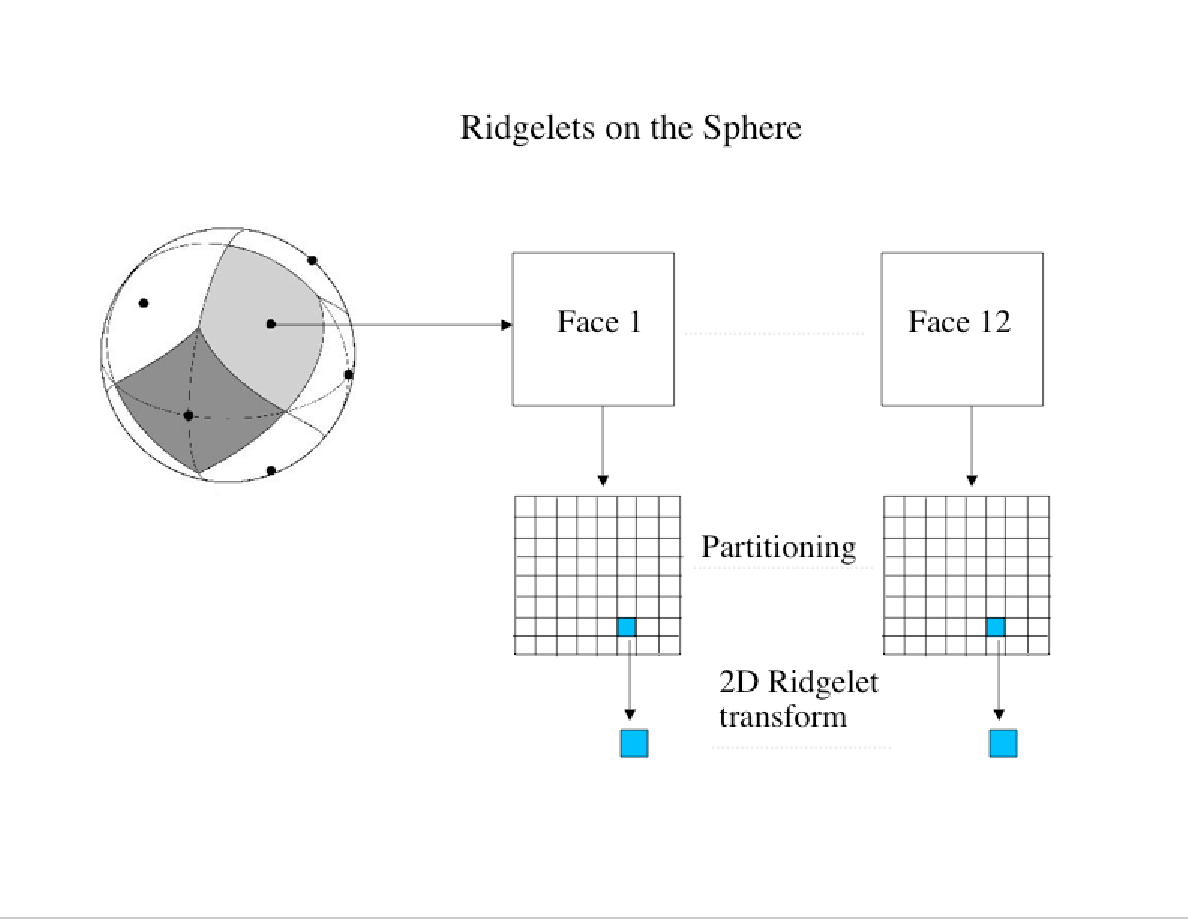
\includegraphics[height = 5 in]{fig_flowgraph_ridgelet_sphere.pdf}
\centerline{
\hbox{
\psfig{figure=fig_flowgraph_ridgelet_sphere.pdf,bbllx=1.5cm,bblly=9cm,bburx=18.5cm,bbury=19cm,height=8cm,width=13.6cm,clip=}
}}
\caption{Flowgraph of the Ridgelet Transform on the Sphere.}
\label{Figure:rid_sphere}
\end{figure*}

\begin{figure*}
% \centering
% 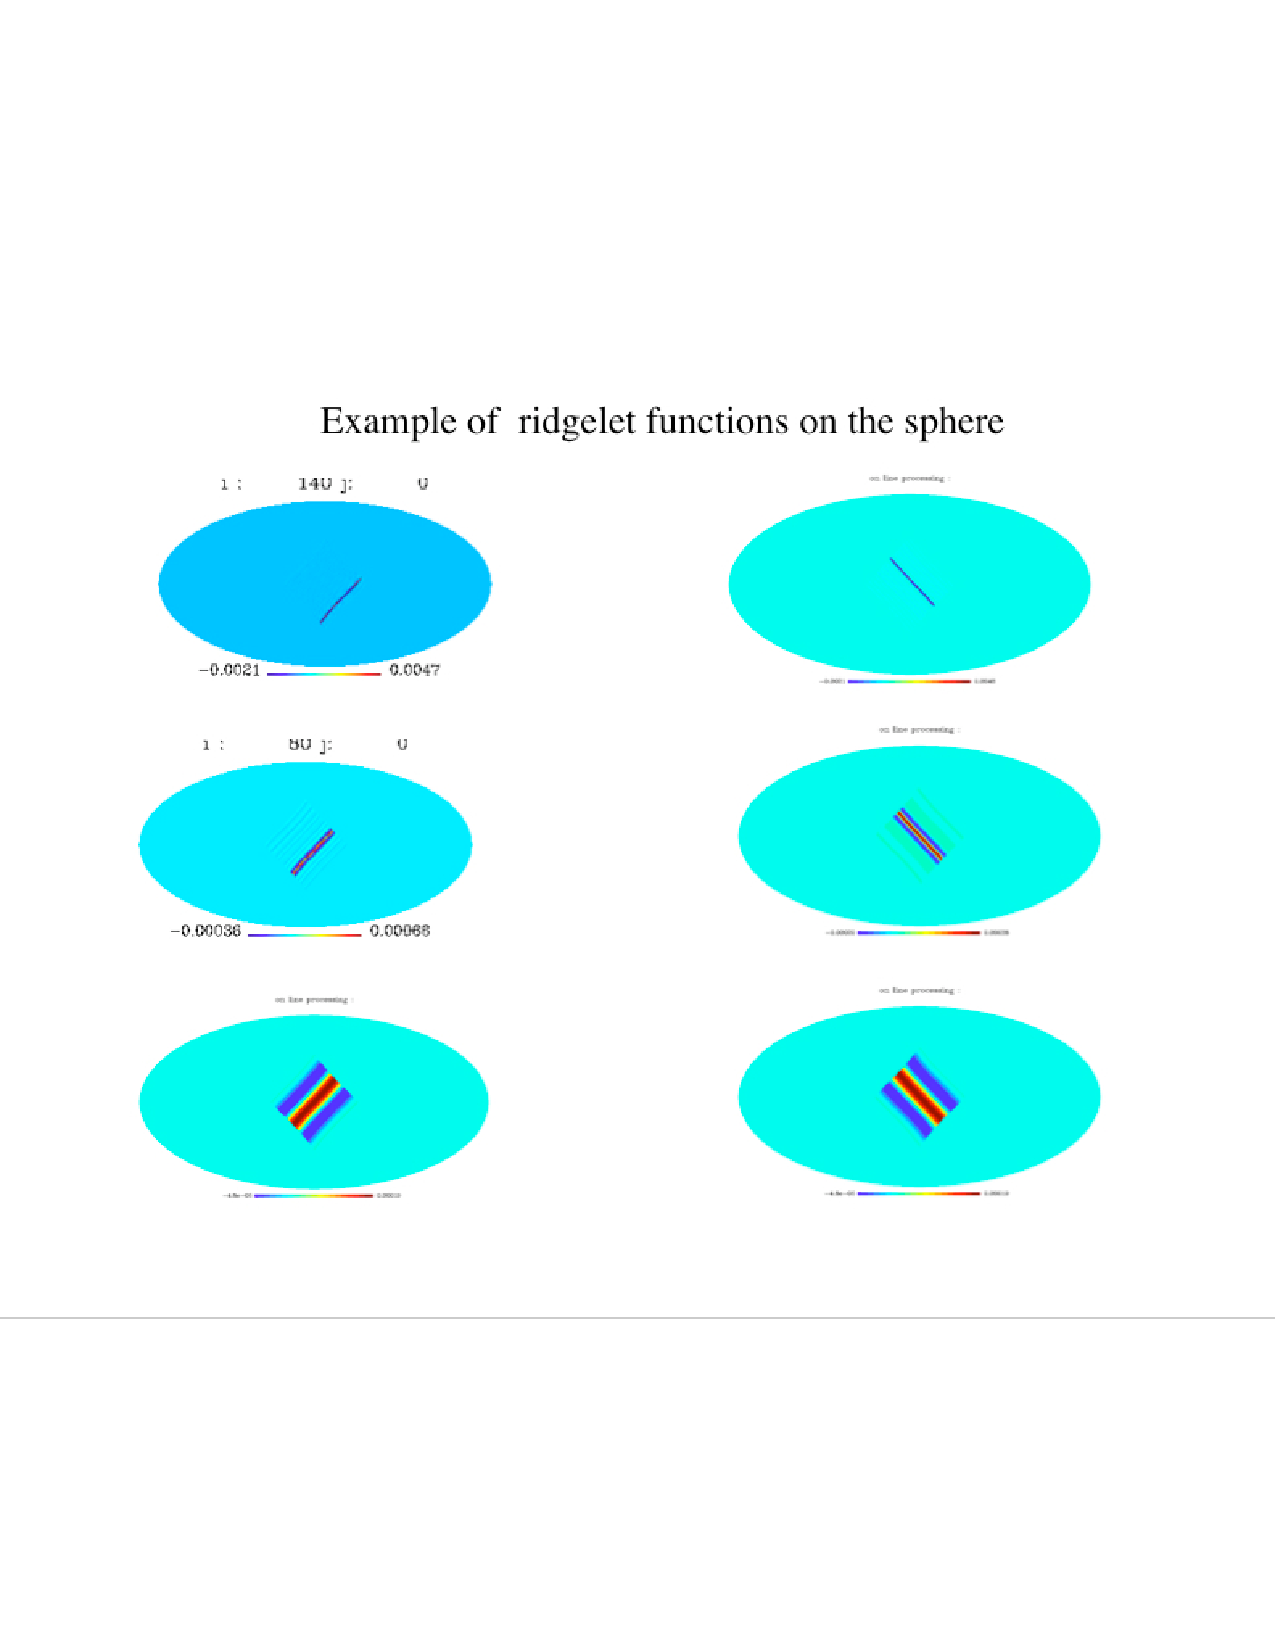
\includegraphics[height = 5 in]{fig_back_rid_sphere.pdf}
\centerline{
\hbox{
% \psfig{figure=fig_back_rid_sphere.ps,bbllx=0.5cm,bblly=7.5cm,bburx=21.5cm,bbury=19.5cm,height=6cm,width=9.5cm,clip=}
\psfig{figure=fig_ridssr.pdf,bbllx=0.5cm,bblly=7.5cm,bburx=21.5cm,bbury=20cm,height=6cm,width=9.5cm,clip=}
}}
\caption{Backprojection of a ridgelet coefficient at different scales and orientations.
{ Each map is obtained by setting all ridgelet coefficients to zero but one, and applying an inverse ridgelet transform. Depending on 
the scale and the position of the non zero ridgelet coefficient, the reconstructed image presents a feature with a given width and a 
given orientation.}}
\label{Figure:back_rid}
\end{figure*}
 

\subsection{Algorithm}
The curvelet transform algorithm on the sphere is as follows:
\begin{enumerate}
\item apply the isotropic wavelet transform on the sphere with $J$ scales,
\item set the block size $B_1 = B_{min}$,
\item for $j = 1, \ldots, J$ do,
\begin{itemize}
\item partition the subband $w_j$ with a block size $B_j$ and apply the digital ridgelet transform to each block,
\item if $j \mbox{ modulo } 2 = 1$ then $B_{j+1} = 2 B_{j}$,
\item else $B_{j+1} = B_{j}$.
\end{itemize}
\end{enumerate}
The sidelength of the localizing windows is doubled {\em at every other} dyadic subband, hence maintaining the fundamental property of
the curvelet transform which says that elements of length about $2^{-j/2}$ serve for the analysis and synthesis of the $j$-th subband
$[2^j, 2^{j+1}]$. We used the default value $B_{min} = 16$ pixels in our implementation. Finally, Figure~\ref{Figure:cur_sphere} gives 
an overview of the organization of the algorithm.
\begin{figure*}
 % 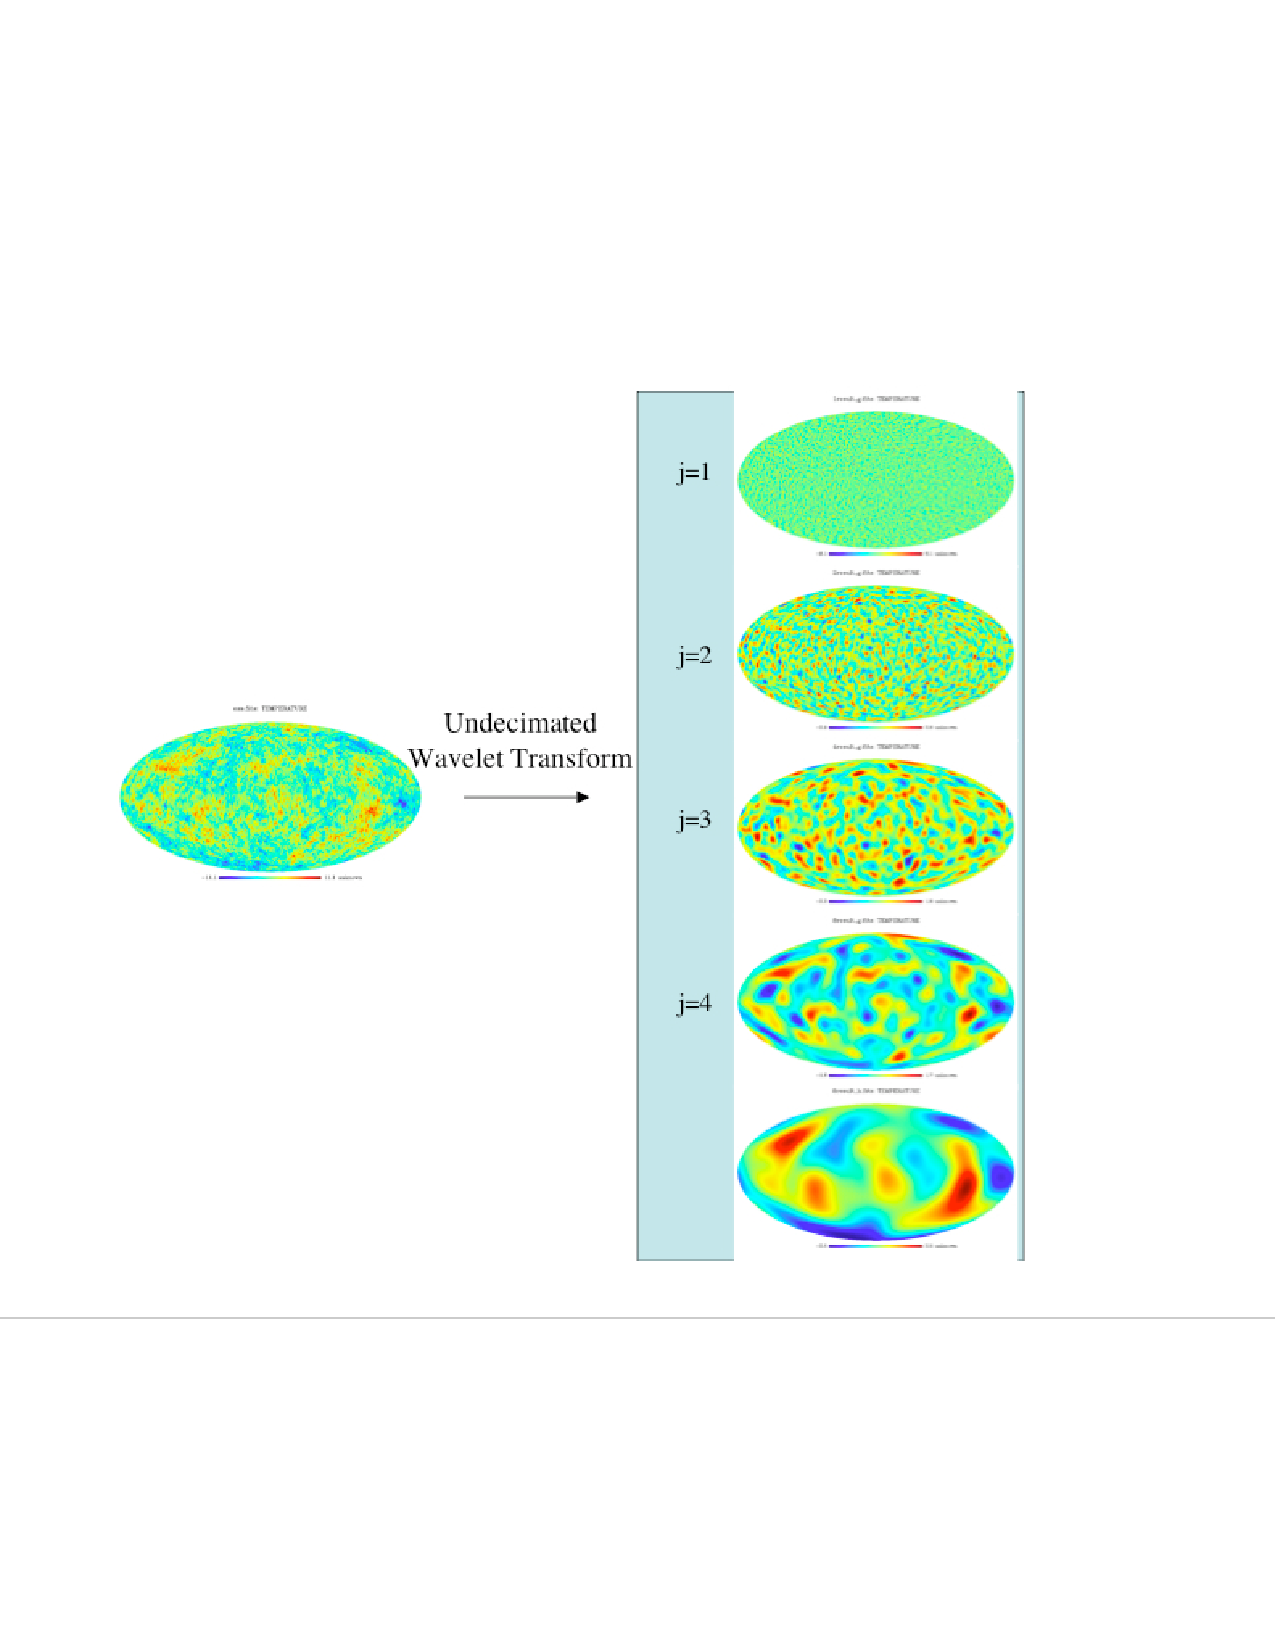
\includegraphics[height=8truecm,width=6truecm]{fig_uwt_sphere.pdf}
% 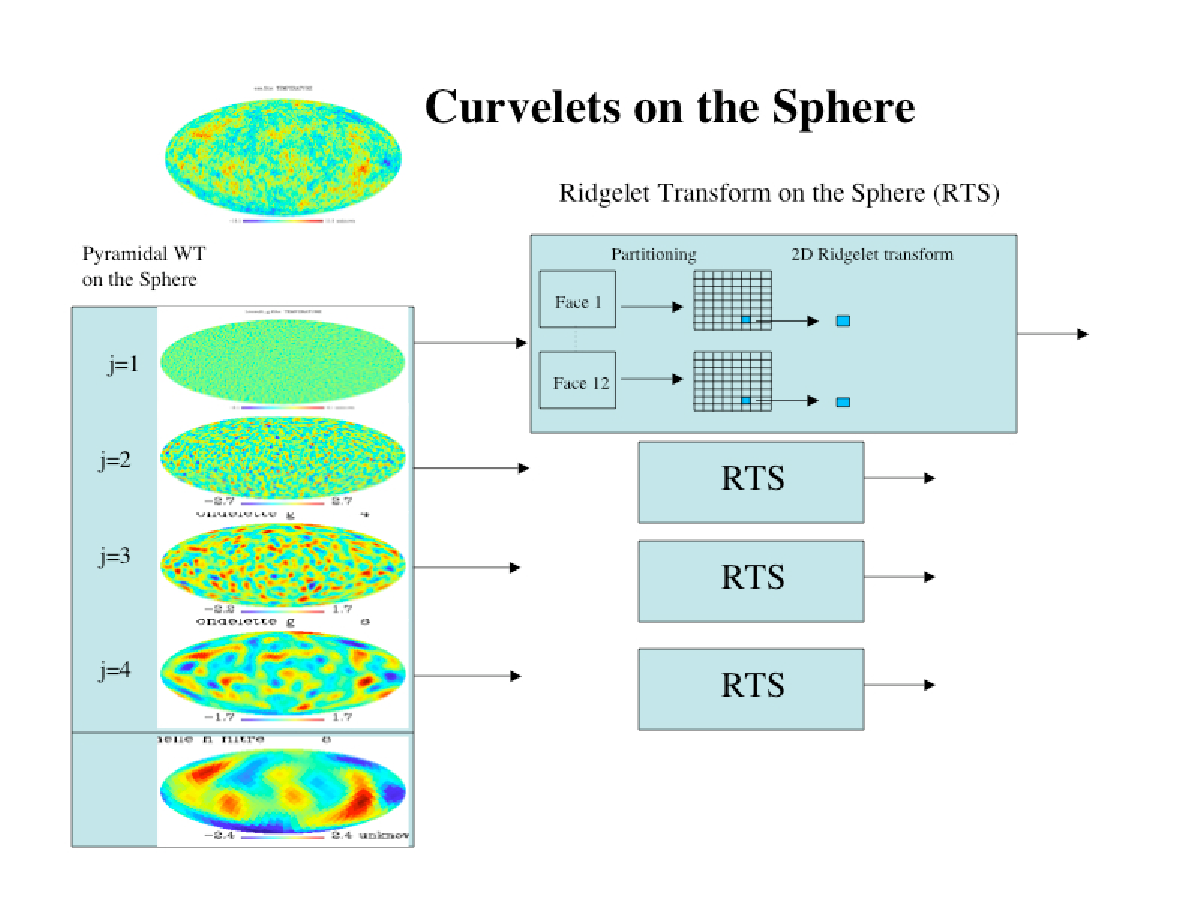
\includegraphics[height = 7 in]{fig_flowgraph_curvelet_sphere.pdf}
\centerline{
\hbox{
\psfig{figure=fig_flowgraph_curvelet_sphere.pdf,bbllx=1cm,bblly=7cm,bburx=20cm,bbury=21cm,height=9cm,width=12cm,clip=}
}}
\caption{Flowgraph of the Curvelet Transform on the Sphere.}
\label{Figure:cur_sphere}
\end{figure*}
\begin{figure*}
% 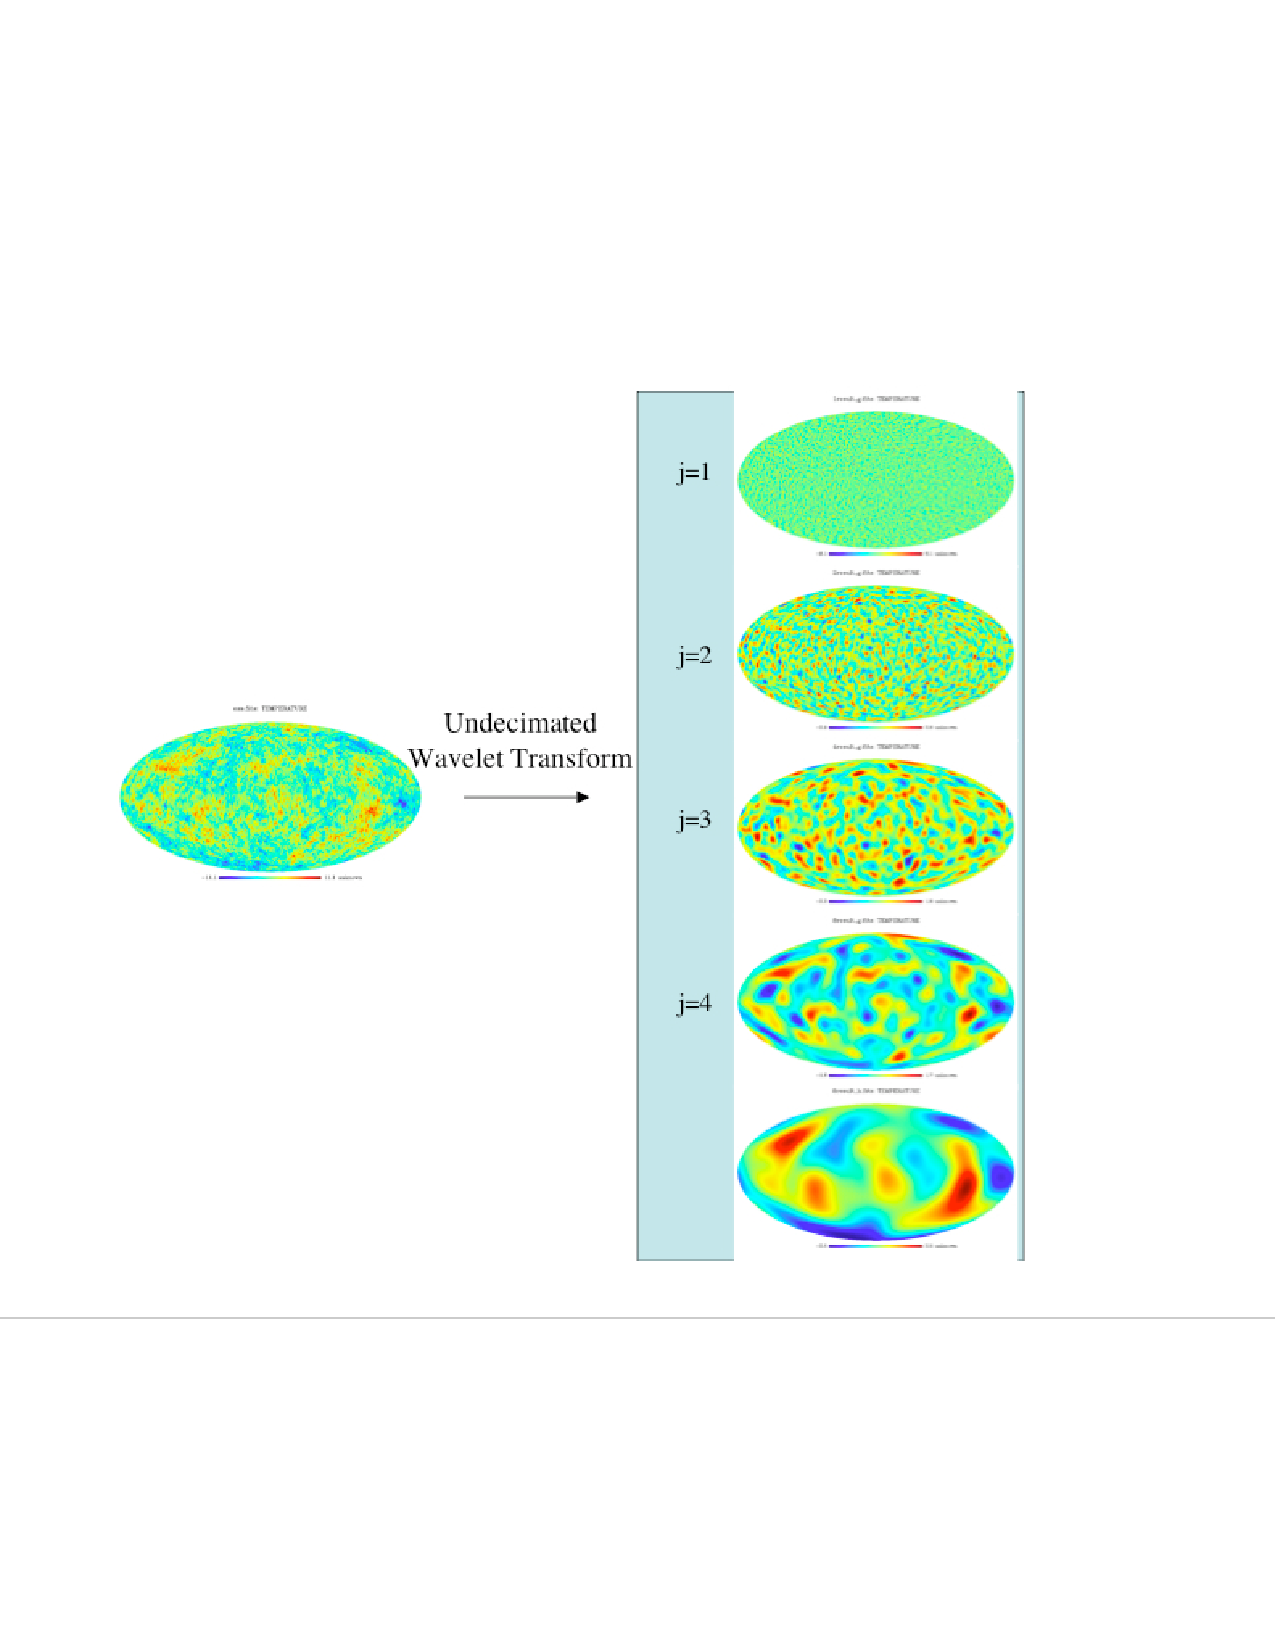
\includegraphics[height=8truecm,width=6truecm]{fig_uwt_sphere.pdf}
% 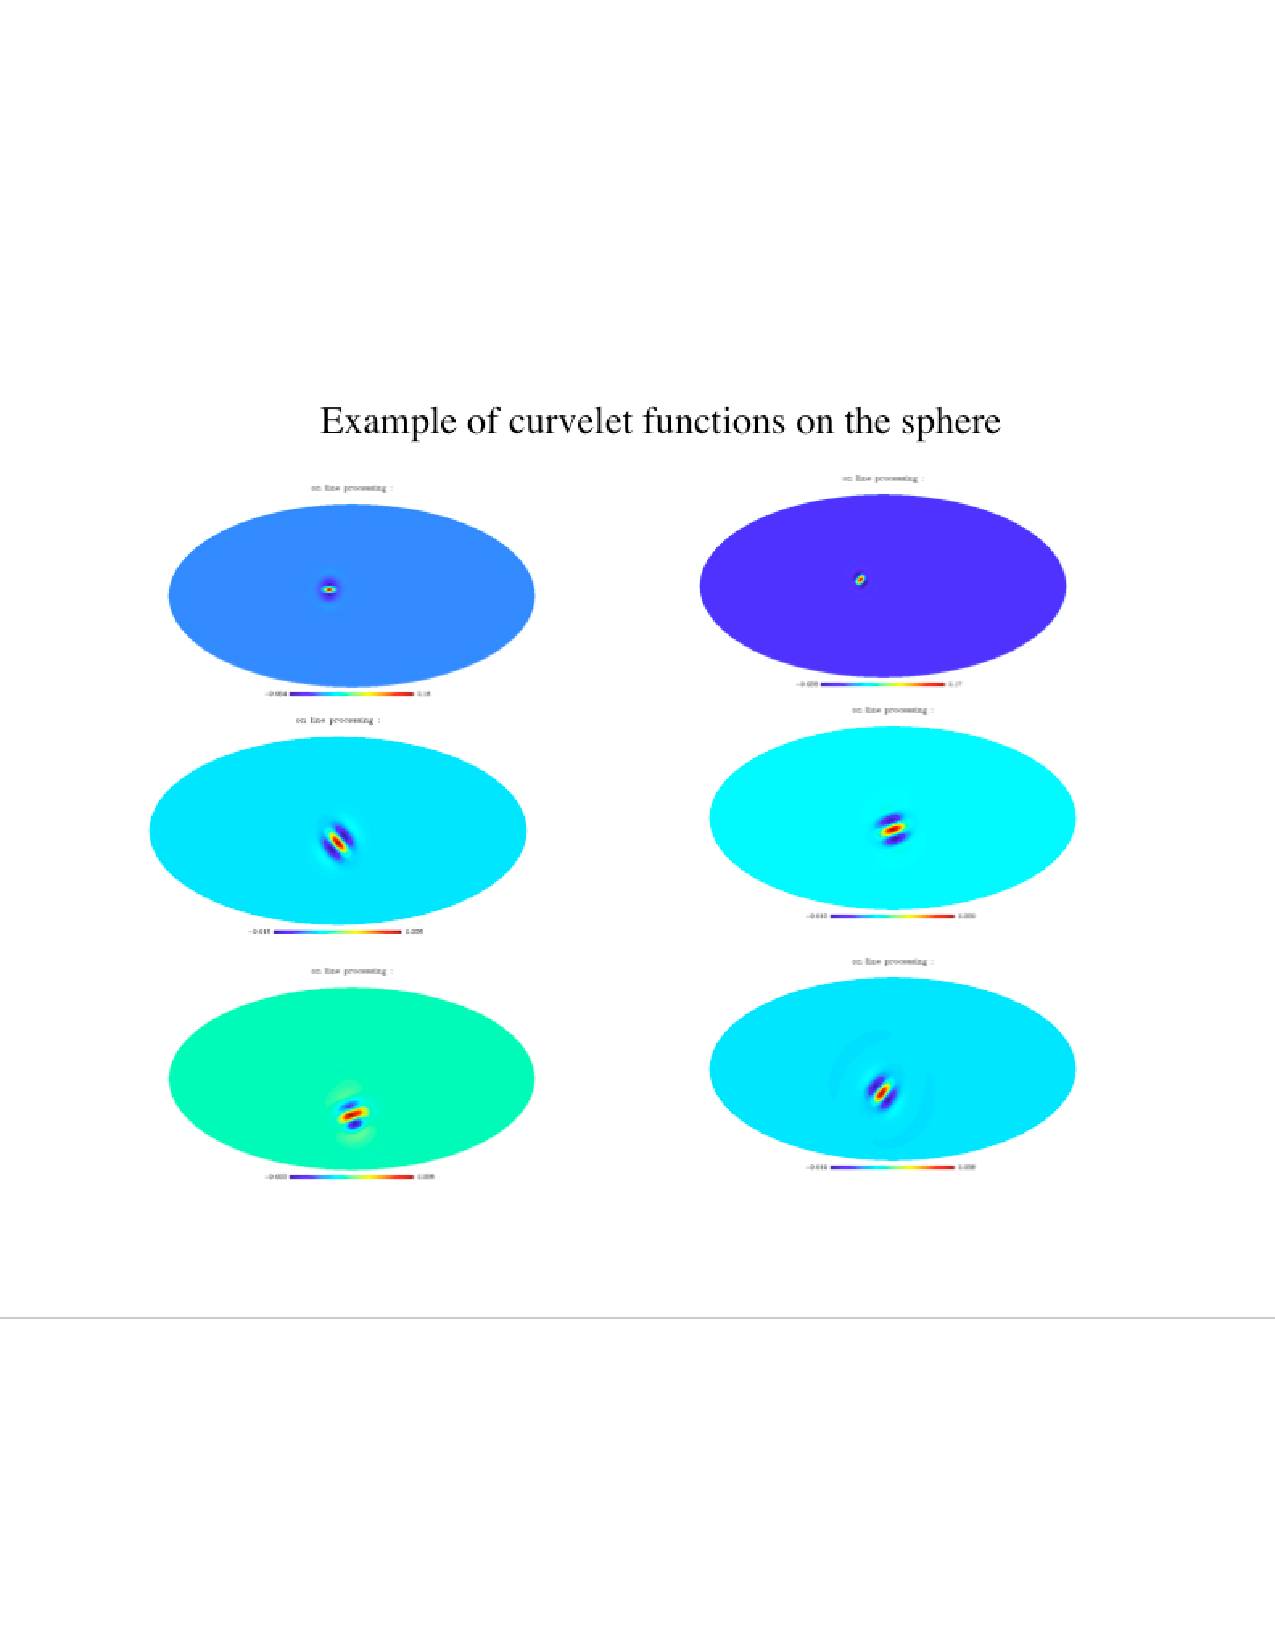
\includegraphics[height = 5 in]{fig_back_cur_sphere.pdf}
\centerline{
\hbox{
\psfig{figure=fig_back_cur_sphere.pdf,bbllx=1cm,bblly=7cm,bburx=20cm,bbury=21cm,height=9cm,width=12cm,clip=}
}}
\caption{Backprojection of a curvelet coefficient at different scales and orientations.
{ Each map is obtained by setting all curvelet coefficients to zero but one, and applying an inverse curvelet transform. 
Depending on the scale and the position of the non zero curvelet coefficient, the reconstructed image presents a feature 
with a given width, length and orientation.}}
\label{Figure:back_cur}
\end{figure*}
Figure~\ref{Figure:back_cur} shows the backprojection of  curvelet coefficients at different scales and orientations.
\index{algorithm!curvelet transform}


\subsection{Pyramidal Curvelet Transform on the Sphere (PCTS)}
\index{curvelet}
\index{curvelet!pyramidal transform}

The CTS is very redundant, which may be a problem for handling huge data sets such as the future PLANCK data. The redundancy 
can be reduced by substituting, in the curvelet transform algorithm, the pyramidal wavelet transform to the undecimated wavelet 
transform. The second step which consists in applying the ridgelet transform on the wavelet scale is unchanged. The pyramidal 
curvelet transform algorithm is:
\begin{enumerate}
\item apply the pyramidal wavelet transform on the sphere with $J$ scales,
\item set the block size $B_1 = B_{min}$,
\item for $j = 1, \ldots, J$ do,
\begin{itemize}
\item partition the subband $w_j$ with a block size $B_j$ and apply the digital ridgelet transform to each block,
\item if $j \mbox{ modulo } 2 = 2$ then $B_{j+1} = B_{j} / 2$,
\item else $B_{j+1} = B_{j}$.
\end{itemize}
\end{enumerate}
In the next section, it is shown how the pyramidal curvelet transform can be used for image filtering.




